%
% This is the LaTeX template file for lecture notes for EE 382C/EE 361C.
%
% To familiarize yourself with this template, the body contains
% some examples of its use.  Look them over.  Then you can
% run LaTeX on this file.  After you have LaTeXed this file then
% you can look over the result either by printing it out with
% dvips or using xdvi.
%
% This template is based on the template for Prof. Sinclair's CS 270.

\documentclass[twoside]{article}
\usepackage{graphicx}
\usepackage{algorithm2e}
\graphicspath{ {./} }
\setlength{\oddsidemargin}{0.25 in}
\setlength{\evensidemargin}{-0.25 in}
\setlength{\topmargin}{-0.6 in}
\setlength{\textwidth}{6.5 in}
\setlength{\textheight}{8.5 in}
\setlength{\headsep}{0.75 in}
\setlength{\parindent}{0 in}
\setlength{\parskip}{0.1 in}

%
% The following commands set up the lecnum (lecture number)
% counter and make various numbering schemes work relative
% to the lecture number.
%
\newcounter{lecnum}
\renewcommand{\thepage}{\thelecnum-\arabic{page}}
\renewcommand{\thesection}{\thelecnum.\arabic{section}}
\renewcommand{\theequation}{\thelecnum.\arabic{equation}}
\renewcommand{\thefigure}{\thelecnum.\arabic{figure}}
\renewcommand{\thetable}{\thelecnum.\arabic{table}}

%
% The following macro is used to generate the header.
%
\newcommand{\lecture}[4]{
   \pagestyle{myheadings}
   \thispagestyle{plain}
   \newpage
   \setcounter{lecnum}{#1}
   \setcounter{page}{1}
   \noindent
   \begin{center}
   \framebox{
      \vbox{\vspace{2mm}
    \hbox to 6.28in { {\bf EE 382V: Social Computing
                        \hfill Fall 2018} }
       \vspace{4mm}
       \hbox to 6.28in { {\Large \hfill Lecture #1: #2  \hfill} }
       \vspace{2mm}
       \hbox to 6.28in { {\it Lecturer: #3 \hfill Scribe: #4} }
      \vspace{2mm}}
   }
   \end{center}
   \markboth{Lecture #1: #2}{Lecture #1: #2}
   %{\bf Disclaimer}: {\it These notes have not been subjected to the
   %usual scrutiny reserved for formal publications.  They may be distributed
   %outside this class only with the permission of the Instructor.}
   \vspace*{4mm}
}

%
% Convention for citations is authors' initials followed by the year.
% For example, to cite a paper by Leighton and Maggs you would type
% \cite{LM89}, and to cite a paper by Strassen you would type \cite{S69}.
% (To avoid bibliography problems, for now we redefine the \cite command.)
% Also commands that create a suitable format for the reference list.
\renewcommand{\cite}[1]{[#1]}
\def\beginrefs{\begin{list}%
        {[\arabic{equation}]}{\usecounter{equation}
         \setlength{\leftmargin}{2.0truecm}\setlength{\labelsep}{0.4truecm}%
         \setlength{\labelwidth}{1.6truecm}}}
\def\endrefs{\end{list}}
\def\bibentry#1{\item[\hbox{[#1]}]}

%Use this command for a figure; it puts a figure in wherever you want it.
%usage: \fig{NUMBER}{SPACE-IN-INCHES}{CAPTION}
\newcommand{\fig}[3]{
			\vspace{#2}
			\begin{center}
			Figure \thelecnum.#1:~#3
			\end{center}
	}
% Use these for theorems, lemmas, proofs, etc.
\newtheorem{theorem}{Theorem}[lecnum]
\newtheorem{lemma}[theorem]{Lemma}
\newtheorem{proposition}[theorem]{Proposition}
\newtheorem{claim}[theorem]{Claim}
\newtheorem{corollary}[theorem]{Corollary}
\newtheorem{definition}[theorem]{Definition}
\newenvironment{proof}{{\bf Proof:}}{\hfill\rule{2mm}{2mm}}

% **** IF YOU WANT TO DEFINE ADDITIONAL MACROS FOR YOURSELF, PUT THEM HERE:

\begin{document}
%FILL IN THE RIGHT INFO.
%\lecture{**LECTURE-NUMBER**}{**DATE**}{**LECTURER**}{**SCRIBE**}
\lecture{7}{November 9}{Vijay Garg}{Cong Wang}
%\footnotetext{These notes are partially based on those of Nigel Mansell.}

% **** YOUR NOTES GO HERE:

% Some general latex examples and examples making use of the
% macros follow.  
%**** IN GENERAL, BE BRIEF. LONG SCRIBE NOTES, NO MATTER HOW WELL WRITTEN,
%**** ARE NEVER READ BY ANYBODY.
\section{Single-peaked preference}

A standard example of cycling, in which there are three people, and three alternatives, A, B, C, and preferences are
\newline
\[X \succ_1 Y \succ_1 Z \]
\[Y \succ_2 Z \succ_2 X \]
\[Z \succ_3 X \succ_3 Y \]
\newline
Suppose that X, Y and Z correspond to amounts of money to spend on education, with X corresponding to a small amount, Y to a medium amount, and Z to a large amount. Then the preferences of voter 1 make sense: she is happiest with the smallest amount, and second-happiest with a medium amount. The preferences of voter 2 also make sense: he is happiest with a medium amount, but if not medium, then he prefers a large amount. The preferences of voter 3, on the other hand, are harder to justify in a simple way: he prefers a large amount, but his second choice is a small amount, with medium coming last. In other words, the first two voters have preferences that can be explained by proximity to a fixed number: each of them has an "ideal" amount that they'd like, and they evaluate the alternatives by how close they come to this ideal. The third voter's preferences can't be explained this way: there's no "ideal" quantity such that both large and small are close to it, but medium isn't. This is not to say that a person couldn't hold these preferences, but they're more unusual.

It turns out that cycling will not be a problem, if people's preferences are aligned in a particular way : if preferences are single-peaked. Let's assume that the \textit{k} alternatives are named $X_1$, $X_2$,..., $X_k$, and that voters all perceive them as being arranged in this order. We say that a voter has a \textbf{single-peaked preference}, if there is no alternative $X_s$ for which both neighboring alternative $X_{s-1}$ and $X_{s+1}$ are ranked above $X_s$. In other words, a voter never prefers two options that lie on opposite sides of a middle option. 

Such preferences are called single-peaked because the condition we impose is equivalent to the following one : each voter i has a top-ranked option $X_t$, and here preferences fall off on both sides of $X_t$ : 
\[X_t \succ_i X_{t+1} \succ_i X_{t+2} \succ_i ... \]
and
\[X_t \succ_i X_{t-1} \succ_i X_{t-2} \succ_i ... \]
Pictorially, this can be represented as in figure 7.1. The example shown there has three voters with preferences
\newline
\[X_1 \succ_1 X_2 \succ_1 X_3 \succ_1 X_4 \succ_1 X_5 \]
\[X_2 \succ_2 X_3 \succ_2 X_4 \succ_2 X_1 \succ_2 X_5 \]
\[X_3 \succ_3 X_2 \succ_3 X_1 \succ_3 X_4 \succ_3 X_5 \]
\newline
and each of the three plots shows one of these sets of individual preferences: In the plots, there is an oval for each alternative, and its height corresponds to its position in the list. As drawn, the single peak in an individual's ranking emerges visually as a peak in the plot.

\begin{figure}[h]
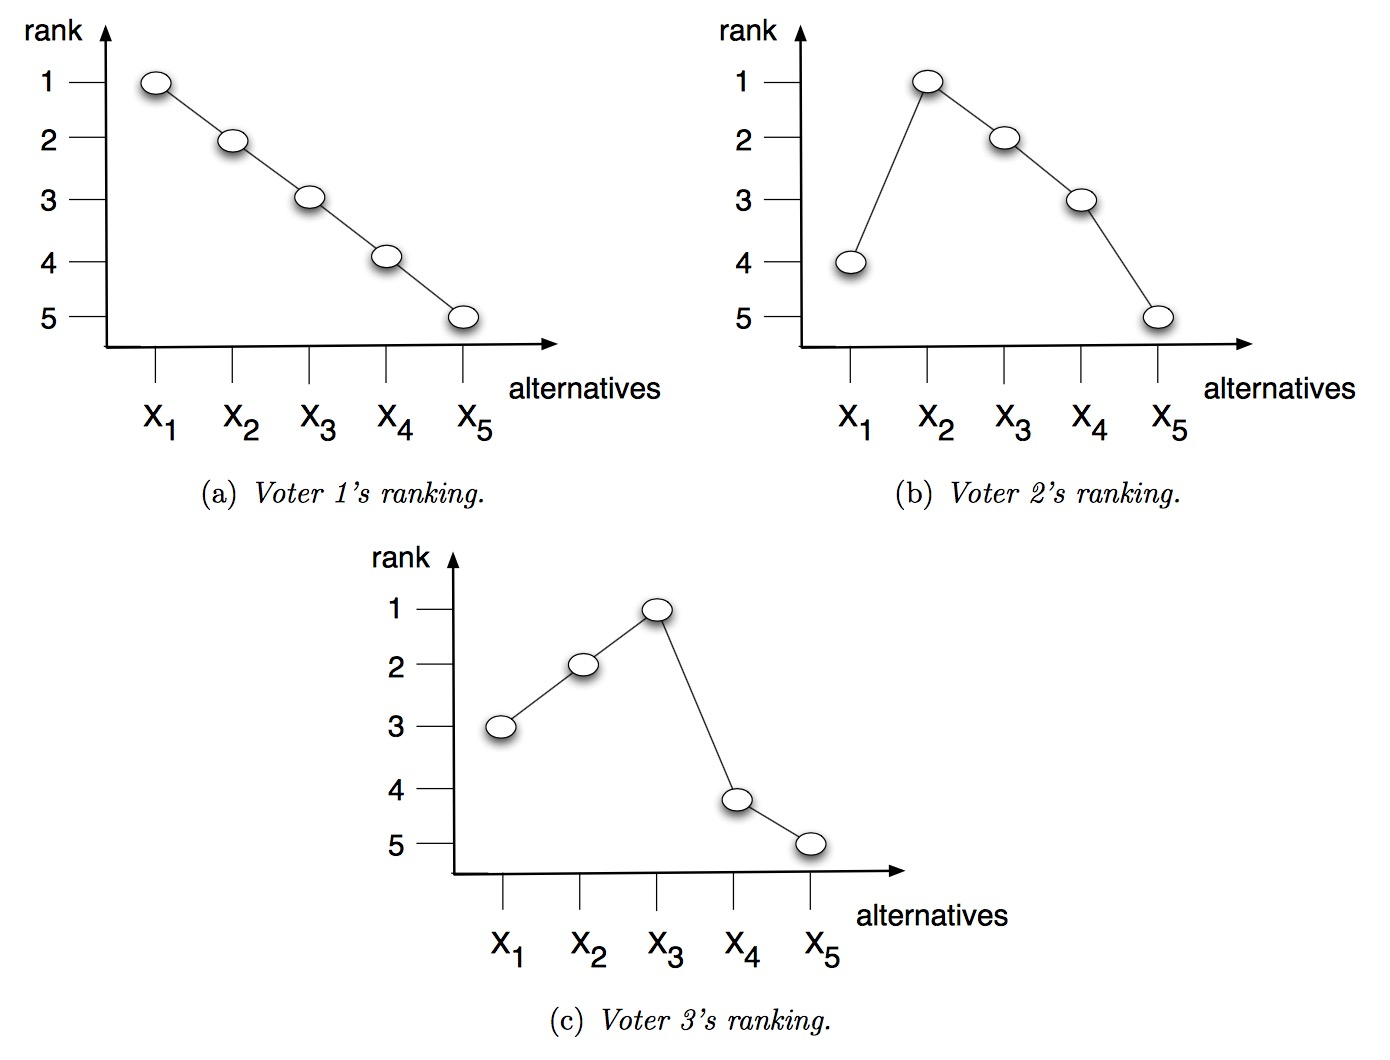
\includegraphics[width=\textwidth]{image1}
\caption{With single-peaked preferences, each voter's ranking of alternatives decreases on both sides of a "peak" corresponding to her favorite choice.}
\label{fig:figure1}
\end{figure}

\section{Median Voter Theorem}

Preferences are single-peaked whenever there is some way of arranging the alternatives along a line so that the graphs of each voter's preferences have just one local maximum. 

\textit{\textbf{Claim}: If all individual rankings are single-peaked, then majority rule applied to all pairs of alternatives produces a group preference relation that is complete and transitive.}

Let's consider the top-ranked alternative for each voter, and sort this set of individual favorites from left to right, along our linear order. Notice that if several voters have the same alternative as their respective individual favorite, then this alternative will appear multiple times in the sorted list: it is fine for the list to have repetitions. Now consider the individual favorite that forms the median of this list - that is, the individual favorite that lies exactly at the halfway point in the sorted order. The median individual favorite is a natural idea to consider as a potential group favorite, since it naturally "compromises" between more extreme individual favorites on either side.

\textit{\textbf{The Median Voter Theorem}: With single-peaked rankings, the median individual favorite defeats every other alternative in a pairwise majority vote.}

\begin{figure}[ht]
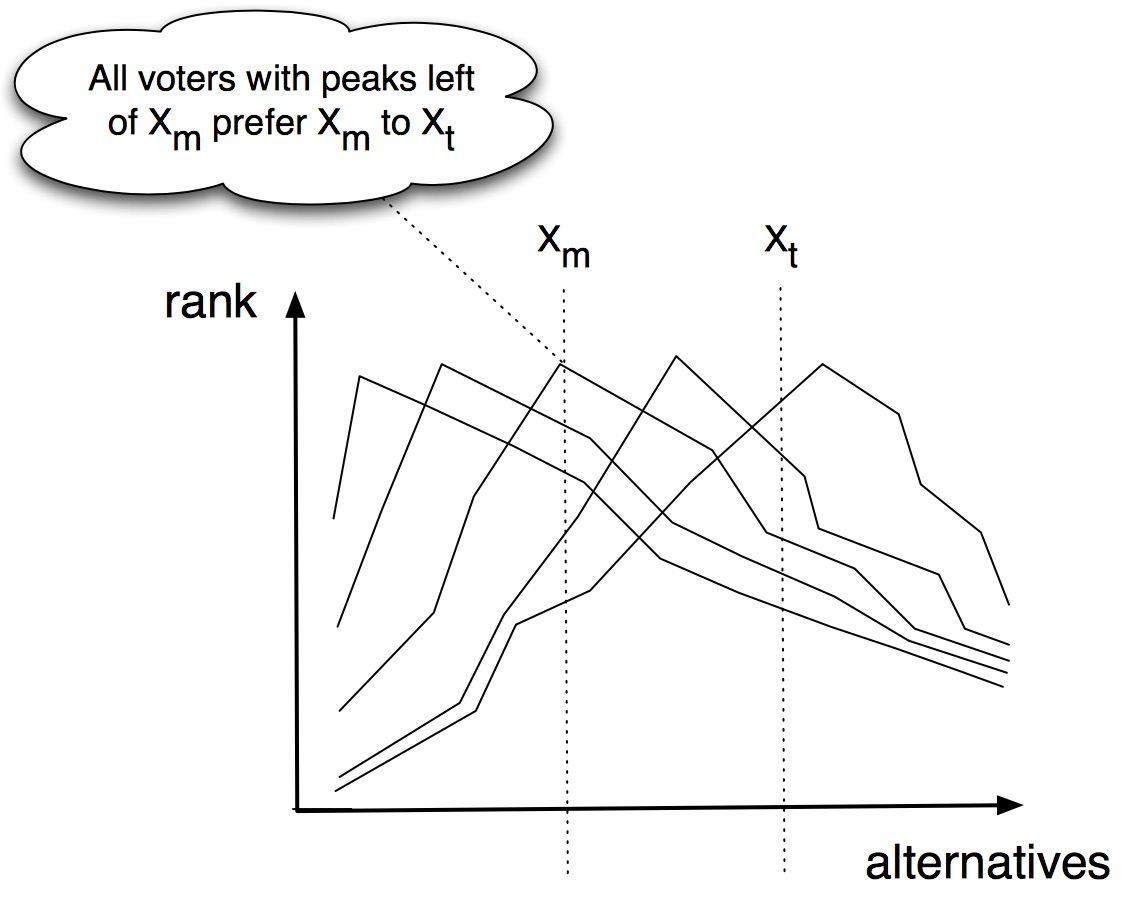
\includegraphics[width=0.7\textwidth]{image2}
\centering
\caption{The proof that the median individual favorite $X_m$ defeats every other alternative $X_t$ in a pairwise majority vote: if $X_t$ is to the right of $X_m$, the $X_m$ is preferred by all voters whose peak is on $X_m$ or to its left. (The symmetric argument applied when $X_t$ is to the left of $X_m$)}
\label{fig:figure2}
\end{figure}

\textbf{Proof: }
\newline
Let $X_m$ be the median individual favorite, and let $X_t$ be any other alternative. Let's suppose that $X_t$ lies to the right of $X_m$ - that is, t $>$ m. (The case in which it lies to the left has a completely symmetric argument.) Let's also order the voters in the sorted order of their individual favorites.
The argument is now depicted schematically in Figure 7.2. The number of voters k is odd, and we know that $X_m$ is in position (k+1)/2 of the sorted list of individual favorites. This means that for everyone in the first (k+1)/2 positions, $X_m$ is either their favorite, or their favorite lies to the left of $X_m$. For each voter in this latter group, $X_m$ and $X_t$ are both on the right-hand "down-slope" of this voter's preferences, but $X_m$ is closer to the peak than $X_t$ is, so $X_m$ is preferred to $X_t$. It follows that everyone in the first (k+1)/2 positions prefers $X_m$ to $X_t$. But this is a strict majority of the voters, and so $X_m$ defeats $X_t$ in a pairwise majority vote. The median individual favorite $X_m$ can always count on gathering a majority of support against any other alternative $X_t$, because for more than half the voters, $X_m$ lies between $X_t$ and each of their respective favorites.

\section{Housing Allocation Problem}

In the "House Allocation Problem" problem, there are n agents and n houses. Each agent $A_i$ initially owns a house $H_i$ and has a completely ranked list of houses. This list is given by \textit{pref}[i][k] which specifies the $k^{th}$ preference of agent i. Thus, \textit{pref}[i][1] = j means that $A_i$ prefers $H_j$ as his top choice. The goal is to come up with an optimal house allocation defined as an allocation such that each agent has a house and no subset of agents can improve the satisfaction of agents in this subset by exchanging houses within the subset.

\subsection{Top Trading Cycles Algorithm }

We will give a simple and intuitive algorithm that will achieve these goals, the "Top Trading Cycles" algorithm.

\begin{algorithm}[H]
\SetAlgoLined
 input: n agents with strict preferences ordering over all the houses ($\succ_1$,...,$\succ_n$)\;
 Let $S_1$ be the set of all agents. Set a counter t = 1\;
 \While{ size of $S_t$ $>$ 0}{
  Construct a graph $G_t$ = ($V_t$, $E_t$) where $V_t$ = $S_t$ and for each (\textit{i}, \textit{j}) $\epsilon$ $E_t$ if and only if $h_j$ $\succ_i$ $h_k$ for all other \textit{k} $\epsilon$ $V_t$. This is the graph that results when every agent points to their most preferred house. And each agent is in at most one cycle \;
  Find any cycle $C_t$ in $G_t$ and for every directed edge (\textit{i}, \textit{j}) $\epsilon$ $C_t$, we assign the entire cycle their most preferred houses, put (\textit{i}, \textit{j}) in map \textit{m}, which means remove the agent from the market with her assigned house \;
  Set $S_{t+1}$ = $S_t$ and for each \textit{i} : (\textit{i}, \textit{j}) $\epsilon$ $C_t$, set $S_{t+1}$ = $S_{t+1}$ - {i}. Increment t (t = t+1) \;
 }
 \caption{Top Trading Cycles Algorithm}
\KwResult{\textit{m}}
\end{algorithm}

\textbf{Lemma} \textit{In each graph $G_t$ constructed by the algorithm, there is at least one cycle $C_t$, and every agent is part of at most one cycle.}

\textbf{Proof}

This follows simply because by construction, $G_t$ is a directed graph in which every vertex has out-degree exactly one. So by starting at any vertex and following edges forward, we must find a cycle, we cannot get stuck, since there is always an outgoing edge, and hence must repeatedly visit some vertex.

\textbf{Claim} \textit{The top trading cycle algorithm terminates with a stable allocation.}

\textbf{Proof}

Suppose there is some trading coalition S with respect to the final allocation. Let $N_1$ be the set of people removed in the first stage. No one in $N_1$ can be part of S, because they all received their favorite items, so they cannot improve by any swap. Let $N_2$ be the set of people removed in the second stage. Each of these people gets their favorite item not owned by anyone in $N_1$. So the only way they could improve is by trading with someone in $N_1$, but since none of those people belong to S, they cannot improve by trading with anyone in S. This can be repeated for people in $N_3$, $N_4$... to show that no one can belong to S. Thus the assumption that there is a trading coalition is false, which means the allocation is stable.

\subsection{Example}

Consider 4 agents with the following preference ordering over each other's houses:
\[\succ_1: 2 \succ 3 \succ 1 \succ 4 \]
\[\succ_2: 1 \succ 3 \succ 2 \succ 4 \]
\[\succ_3: 1 \succ 2 \succ 3 \succ 4 \]
\[\succ_4: 2 \succ 3 \succ 4 \succ 1 \]

\begin{figure}[ht]
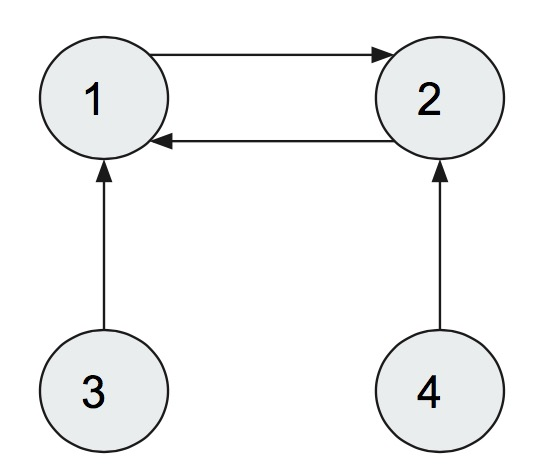
\includegraphics[width=0.3\textwidth]{image3}
\centering
\caption{remove (1,2) and (2,1)}
\label{fig:figure3}
\end{figure}

\begin{figure}[ht]
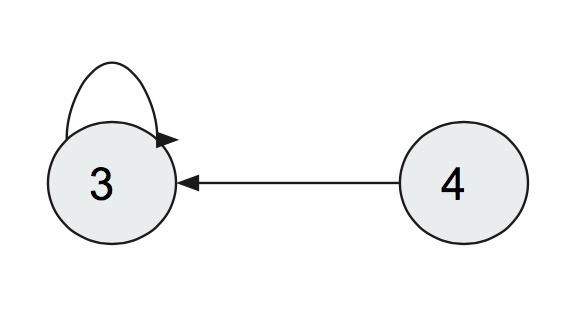
\includegraphics[width=0.3\textwidth]{image4}
\centering
\caption{remove (3,3)}
\label{fig:figure4}
\end{figure}

\begin{figure}[ht]
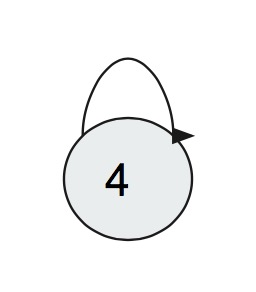
\includegraphics[width=0.2\textwidth]{image5}
\centering
\caption{remove (4,4)}
\label{fig:figure5}
\end{figure}

So the result is ($A_1$, $H_2$), ($A_2$, $H_1$), ($A_3$, $H_3$), ($A_4$, $H_4$) 


\section*{References}
\beginrefs
\bibentry{1}{\sc David Easley} and {\sc Jon Kleinberg},
Networks, Crowds, and Markets: Reasoning about a Highly Connected World.
{\it Cambridge University Press\/}~(2010),
pp.~750--756.

\bibentry{2} lecture slides from UMass.
{\it https://people.cs.umass.edu/~sheldon/teaching/mhc/cs312/2014sp/Slides/top-trading-cycles.pdf\/}~(2014).

\bibentry{3} lecture slides from UPenn.
{\it https://www.cis.upenn.edu/~aaroth/courses/slides/agt17/lect11.pdf\/}~
\endrefs

\end{document}





